% ══════════════════════════════════════════════════════════════════════════════
% 教育部獎學金申請：將各份文件之 PDF 依序合併為單一 PDF（附書籤）。
%   1. 研究計畫書                        01_research_proposal/proposal.pdf     （保留原頁碼）
%   2. 研究優異表現證明                  02_research_excellence/excellence.pdf （單頁，無頁碼）
%   3. 其他有利審查文件：個人學經歷摘要  03_other_documents/profile.pdf        （單頁，無頁碼）
% 各份文件須先編譯；在本資料夾執行 `make` 會依序編譯全部文件再合併。
% ══════════════════════════════════════════════════════════════════════════════
\documentclass{article}

\usepackage{pdfpages}
\usepackage[hidelinks, bookmarksopen]{hyperref}

% Pages are inserted as-is: the proposal keeps its own page numbers, the
% single-page documents have none, and no page number is added here.
\pagestyle{empty}

\begin{document}

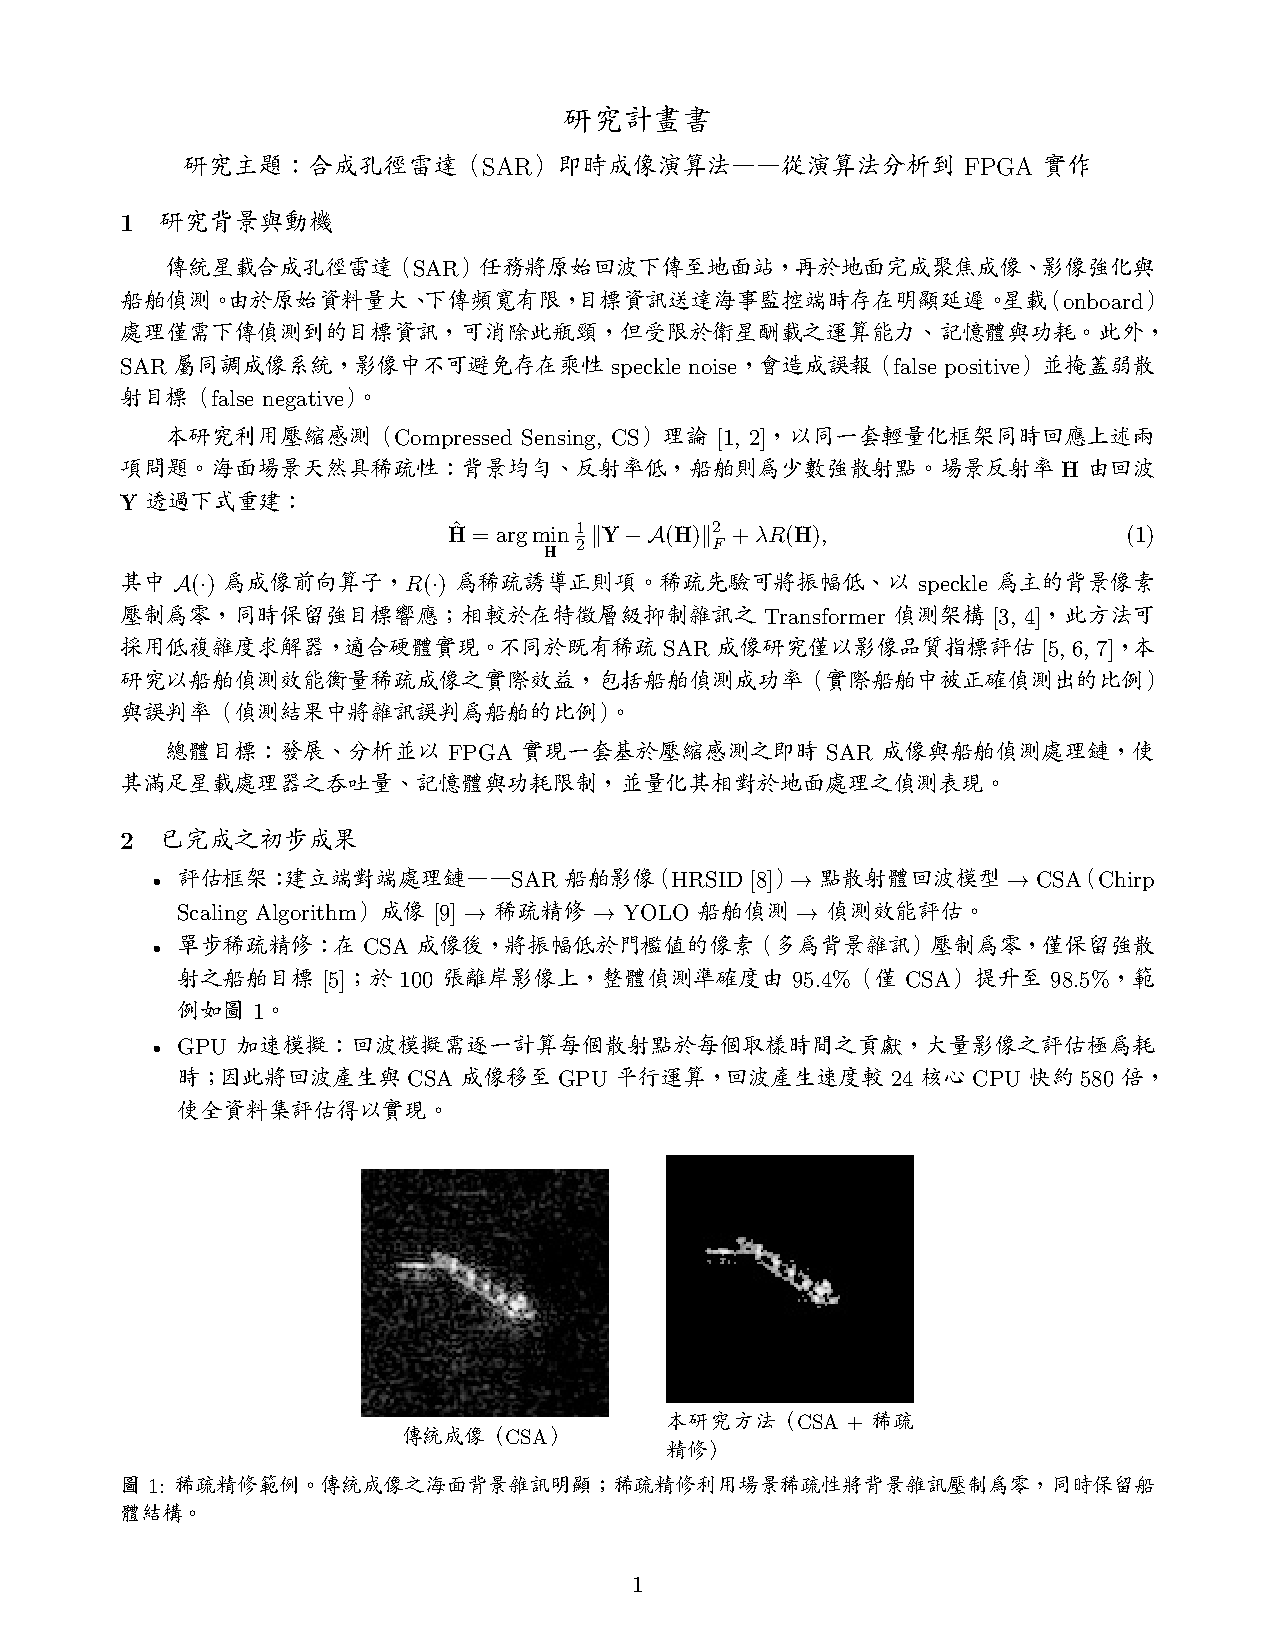
\includepdf[pages=-, addtotoc={1, section, 1, 研究計畫書, proposal}]
  {01_research_proposal/proposal.pdf}

\includepdf[pages=-, addtotoc={1, section, 1, 研究優異表現證明, excellence}]
  {02_research_excellence/excellence.pdf}

\includepdf[pages=-, addtotoc={1, section, 1, 其他有利審查文件：個人學經歷摘要, profile}]
  {03_other_documents/profile.pdf}

\end{document}
